\section{Computational Bottlenecks}

As stream programs are a prime target for parallelization, it is
important to understand the real and artificial bottlenecks to
achieving high parallel performance.  In this section, we use the term
``stateful'' to refer to filters that retain mutable state from one
execution to the next; filters containing only read-only state are
classified as ``stateless''.  Stateless filters are amenable to data
parallelism, as they can be replicated any number of times to work on
different parts of the input stream~\cite{gordon-asplos06}.  However,
stateful filters must be run in a serial fashion, as there is a
dependence from one iteration to the next.  While separate stateful
filters can be run in a task-parallel or pipeline-parallel mode, the
serial nature of each individual filter represents an eventual
bottleneck to the parallel computation.

% Peeking is widely used for a variety of sliding window computations.
% Without peeking, such computations would often introduce a stateful
% bottleneck in the program.
\myitem {\slidingwindows} Twenty two benchmarks -- and more than half
of the realistic applications -- contain at least one filter that
peeks.  (That is, these filters declare a peek rate larger than their
pop rate, and thus implement a sliding window computation.
%examining some items that are not dequeued from the input
%channel until a later execution.  
We do not count filters that merely call the peek primitive, as those
items may be popped during the same execution.)  Benchmarks contain up
to 4 filter types that peek; in programs with any peeking, an average
of 10 peeking filters are instantiated.
\label{sec:peeking}

While peeking is used for many purposes, there are a few common
patterns.  The most common is that of an FIR filter, where a filter
peeks at N items, pops one item from the input, and pushes a weighted
sum to the output.  FIR filters account for slightly less than half
(15 out of 35) of the peeking filter declarations.  They are
responsible for all of the peeking in 7 benchmarks (3GPP, OFDM,
Filterbank, TargetDetect, DToA, Oversampler, RateConvert) and some of
the peeking in 3 others (Vocoder, ChannelVocoder, FMRadio).

A second pattern of peeking is when a filter peeks at exactly one item
beyond its pop window.  An example of this filter is a difference
encoder, as used in the JPEG transcoder and Vocoder benchmarks.  On
its first execution, this filter's output is the same as its first
input; on subsequent executions, it is the difference between
neighboring inputs.  As illustrated in
Figure~\ref{fig:diff-stateless}, a difference encoder can be written
as a stateless filter using peeking (and prework, as described later).
Otherwise, the filter is forced to maintain internal state, as
illustrated in Figure~\ref{fig:diff-stateful}.  Across our benchmark
suite, this pattern accounts for more than one quarter (10 out of 35)
of the peeking filter declarations.  It accounts for all of the
peeking in 4 benchmarks (Mosaic, JPEG decode, JPEG transcode, HDTV,
BubbleSort) and some of the peeking in 2 others (Vocoder, FMRadio).
It should be noted that the operation performed on the two items is
sometimes non-linear; for example, Mosaic determines the correlation
between successive frames; FMRadio performs an FM demodulation and
HDTV performs an XOR.

The remaining peeking filters (10 out of 35) perform various
sliding-window functions.  For example, MP3 reorders and adds data
across large (>1000 item) sliding windows;
%GSM performs a coarse-grained (pop 40, peek 80, pop 160) sliding
%duplication in preparation for other steps;
802.11 and SampleTrellis do short (3-7 item) bit-wise operations as
part of an error-correcting code; Vocoder and Audiobeam use peeking to
skip N items (by default 1-14), analogous to an inverse delay;
ChannelVocoder performs a sliding autocorrelation and threshold across
N items (by default 100).

Without peeking, the filters described above would have to be written
in a stateful manner, as the locations peeked would be converted to
internal states of the filter.  This inhibits parallelization, as
there is a dependence between successive filter executions.  To
estimate the resulting performance impact,
Table~\ref{tab:lang-benchmarks-filters} lists the approximate amount
of work in the most computationally-heavy peeking filter in each
benchmark.  For 11 benchmarks, this work represents a significant
fraction of the program load (minimum 3.1\%, median 8\%, maximum
97.6\%) and would represent a new bottleneck in a parallel
computation.  For 8 benchmarks, the state that would be introduced by
peeking is dwarfed by state already present for other reasons.  For
the remaining 3 benchmarks, the peeking filters represent a negligible
(0.1\%) fraction of work.

%{Prework functions are useful for expressing startup conditions, and
%  for eliminating associated state.}
\myitem{\startup} The prework function allows a filter to have
different behavior on its first invocation.  This capability is
utilized by 15 benchmarks, in 20 distinct filter declarations (results
not shown in table).
\label{sec:startup}

The most common use of prework is for implementing a delay; on the
first execution, the filter pushes N placeholder items, while on
subsequent executions it acts like an Identity filter.  A delay is
used in 8 benchmarks (MPD, HDTV, Vocoder, 3GPP, Filterbank, DToA,
Lattice, and SampleTrellis).  Without prework, the delayed items would
need to be buffered within the filter, introducing a stateful
bottleneck to the computation.

\begin{figure}[t!]
\vspace{-6pt}
\centering
\eightpoint
\begin{verbatim}
int->int filter DifferenceEncoder_Stateless {

    prework push 1 peek 1 {
        push(peek(0));
    }

    work pop 1 peek 2 push 1 {
        push(peek(1)-peek(0));
        pop();
    }
}
\end{verbatim}
\vspace{-10pt}
\caption{Stateless version of a difference encoder, using peeking
and prework.\protect\label{fig:diff-stateless}}
\end{figure}

Other benchmarks use prework for miscellaneous startup conditions.  As
mentioned previously, the difference encoder in
Figure~\ref{fig:diff-stateless} relies on prework (used in JPEG
transcoder and Vocoder), as does the analogous difference decoder
(used in JPEG decoder).  The MPEG2 encoder and decoder use prework in
filters relating to picture reordering, while GSM and CRC use prework
for functions analogous to delays.  Prework is also used for
initialization in MPD, HDTV, and 802.11.

\footnotetext[1]{Only non-comment, non-blank lines of code are
  counted.  Line counts do not include libraries used, though other
  statistics do consider both the application and its libraries.}
\footnotetext[2]{Some helper functions in FAT, HDTV, and SampleTrellis
  remain untranslated from the Java-based StreamIt syntax.}
\footnotetext[3]{The graphics pipelines are described in more detail
  elsewhere~\cite{chen-graphics05}.}  
\footnotetext[4]{Due to the large size of MPEG2, splitjoins
  replicating a single filter are automatically collapsed by the
  compiler prior to gathering statistics.}
\footnotetext[5]{Source and sink nodes that generate synthetic input,
  check program output, or perform file I/O are not counted as
  stateful.}
\footnotetext[6]{Work is given as an estimated fraction of the overall
  program, as calculated by a static analysis.  Actual runtimes may
  differ by 2x or more.  Work estimates are not available (N/A) given
  dynamic rates (MPEG2, Mosaic, Graphics pipelines) or external Java
  routines (HDTV, SampleTrellis).}

%% Stateful filters are less common than we expected, though are
%% nonetheless required for complete expression of many algorithms.
%% Further state could be eliminated via new language constructs,
%% compiler analyses, or programmer interventions.
\myitem{\stateful} After effective use of peeking and prework
primitives, one quarter (17 out of 67) of the benchmarks still contain
one or more filters with mutable state.  There are 49 stateful filter
types in the StreamIt benchmark suite, representing approximately 6\%
of the total filters.
%While other researchers have noted that stream
%programs are rich in data parallelism~\cite{imagine03ieee}, we
%nonetheless expected to see a greater proportion of filters that
%retained mutable state between execution steps.  
The heaviest stateful filter in each benchmark ranges from 0.3\% to
42.4\% (median 4.7\%) of the overall work, representing an eventual
bottleneck to parallelization.
\label{sec:stateful}

Of the stateful filters, at least 22 (about 45\%) represent
fundamental feedback loops that are an intrinsic part of the
underlying algorithm.  Filters in this category include the
bit-alignment stage of MPEG encoding, which performs data-dependent
updates to the current position; reference frame encoding in MPEG
encoder, which sometimes stores information about a previous frame;
the parser in MPEG decoder, which suspends and restores its current
control flow position in order to maintain a constant output rate; the
motion prediction, motion vector decode, and picture reordering stages
of MPEG decoder, which contain data-dependent updates of various
buffers; the pre-coding and Ungerboeck encoding stages of HDTV, which
are simple feedback loops; the Ungerboeck decoding stage of HDTV (and
analogously in SampleTrellis) which mutates a persistent lookup table;
multiple feedback loops in GSM; an accumulator, adaptive filter, and
feedback loop in Vocoder; incremental phase correction in OFDM; and
persistent screen buffers in the graphics pipelines.

\begin{figure}[t!]
\vspace{-6pt}
\eightpoint
\begin{verbatim}
int->int filter DifferenceEncoder_Stateful {
    int state = 0;

    work pop 1 push 1 {
        push(peek(0)-state);
        state = pop();
    }
}
\end{verbatim}
\vspace{-10pt}
\caption{Stateful version of a difference encoder, using 
internal state.\protect\label{fig:diff-stateful}}
\end{figure}

The remaining filters classified as stateful may be amenable to
additional analyses that either eliminate the state, or allow
restricted parallelism even in the presence of state.  Twenty filters
contain state due to message handlers, in which a filter field is
modified in response to a message; however, if the message sender is
not data-dependent on the output of the filter, this state does not
restrict parallelism.  Nine filters contain states that track complex
induction variables, such as a cyclic counter or a position within a
two-dimensional array.  Additional states are due to writing a filter
at a fine level of granularity, in which temporary states are stored
rather than being carried to completion.  Further analysis of these
patterns is available in our full report~\cite{thies-thesis}.

%% The largest category of such filters are those in which the state
%% variables are modified only by message handlers.  Whether such
%% messages represent a genuine feedback loop depends on whether the
%% filter sending the message is data-dependent on the outcome of the
%% filter receiving the message.  Even if a feedback loop does exist,
%% it may be possible to exploit bounded parallelism due to the
%% intrinsic delay in that loop, or speculative parallelism due to the
%% infrequent arrival of most teleport messages.  In our benchmarks,
%% there are 16 filters in which the state is mutated only by message
%% handlers; they originate from MPEG encoder, MPEG decoder, Mosaic,
%% and both versions of FHR.  There are also 4 additional filters
%% (drawn from MPEG encoder, MPEG decoder, and Mosaic) in which
%% message handlers account for some, but not all, of the state.

%% A second category of state which could potentially be removed is
%% that of induction variables.  Several filters keep track of how
%% many times they have been invoked, in order to perform a special
%% action every N iterations.  For example, MPEG encoder counts the
%% frame number in assigning the picture type; MPD and Radar (fine
%% grained version) count the position within a logical vector while
%% performing FIR filtering; and SampleTrellis includes a noise source
%% that flips a bit every N items.  Other filters keep track of a
%% logical two-dimensional position, incrementing a column counter on
%% every iteration and only incrementing the row counter when a column
%% is complete.  Filters in this category include motion estimation
%% from MPEG encoder, and two filters from MPD.  Other filters in MPD
%% contain more complex induction variables; an accumulator is reset
%% when a different counter wraps-around to zero.  Taken together,
%% there are a total of 9 filters that could become stateless if all
%% induction variables could be converted to a closed form.

%% There are two approaches for eliminating induction variables from
%% filter state.  The first approach is to recognize them automatically
%% in the compiler.  While this is straightforward for simple counters,
%% it may prove difficult for nested counters (tracking both row and
%% column) or co-induction variables (periodically reseting one variable
%% based on the value of another).  The second approach is to provide a
%% new language primitive that automatically returns the current
%% iteration number of a given filter.  This information can easily be
%% maintained by the runtime system without inhibiting parallelization;
%% shifting the burden from the programmer to the compiler would improve
%% both programmability and performance.

%% The third and final category of state that could potentially be
%% removed is that which results from writing a logically
%% coarse-grained filter at a fine level of granularity.  This can
%% result in a filter in which state variables are reset every N
%% executions, corresponding to one coarse-grained execution
%% boundaries.  Such filters can be re-written in a stateless manner
%% by moving state variables to local variables in the work function,
%% and scaling up the execution of the work function to represent N
%% fine-grained iterations.  Such coarsening would eliminate the state
%% in bubble sort, which is reset at boundaries between data sets, as
%% well as a complex periodic filter (LMaxCalc) in MPD.  It would also
%% eliminate many of the induction variables described previously, as
%% they are also periodic.  This approach provides a practical
%% solution for eliminating state, and was employed in translating
%% Radar from the original fine-grained version to a coarse-grained
%% alternative (both of which appear in our benchmark suite).  The
%% drawbacks of this transformation are the effort required from the
%% programmer and also the increased size of the resulting filter.
%% Coarse-grained filters often incur a larger code footprint, a
%% longer compile time, and a less natural mapping to fine-grained
%% architectures such as FPGAs.  While the StreamIt language aims to
%% be agnostic with respect to the granularity of filters, in some
%% cases the tradeoff between writing stateless filters and writing
%% fine-grained filters may need to be iteratively explored to achieve
%% the best performance.

% Feedback loops are uncommon in our benchmarks, but represent
% significant bottlenecks when present.
\myitem {\feedback} While our discussion thus far has focused on
stateful filters, seven benchmarks also contain explicit feedback
loops in the graph structure.  Three additional benchmarks (MPEG2
encoder, Mosaic, and FHR) contain implicit loops due to teleport
messages that are sent upstream (see Section~\ref{sec:messaging}.  Of
the explicit feedback loops, four represent significant bottlenecks to
parallelization (Fib, FHR feedback, H264 subset, CRC), with workloads
ranging from 73\% to 99\% of the overall execution.  The loop in GSM
is shadowed by a stateful filter; the loop in DToA represents only
0.7\% of the runtime; and the loop in Mosaic, while likely a
bottleneck, is difficult to quantify due to dynamic rates.  Unlike
some of the stateful filters, these feedback loops are all intrinsic
to the algorithm and are not subject to automatic removal.  However,
feedback loops can nonetheless afford opportunities for parallelism
due to the delay in the loop -- that is, if items are enqueued along
the feedback path at the start of execution, then they can be
processed in parallel.  Further analysis of these delays is needed to
assess the potential parallelism of feedback loops in our benchmark
suite.

% The state observed can be explained as follows.  Vocoder performs an
% adaptive DFT that uses a stateful decay to ensure stability; it also
% needs to retain the previous output across one iteration within a
% phase transformation.  MPEGDecoder maintains significant state in
% the parser, and also has negligible state in retaining predicted
% motion vectors across one iteration of work.  Radar repeatedly
% operates on long columns of an array requiring special behavior at
% the boundaries; thus, the state tracks the position in the column
% and does some internal buffering.  Radar can be rewritten at a
% coarse level of granularity to eliminate this state.

\section{Scheduling Characteristics}

The semantics of a stream program is that all filters execute
concurrently, limited only by the availability of data on the input
channels (and the availability of space on the output channels).
Thus, it is the role of the compiler to schedule the actual sequence
of filter executions on a given target.  This section describes the
constraints and opportunities of the scheduling process, as informed
by our benchmark suite.

% Neighboring filters often have matched I/O rates
\myitem {\matchedrates} Many of the advanced scheduling strategies for
synchronous dataflow graphs have the highest payoff when the input and
output rates of neighboring filters are mismatched.  For example, the
CD-DAT benchmark (shown in Figure~\ref{fig:cd-dat}) is used in many
studies~\cite{bhattacharya_quasi-static_2000,bhattacharyya_optimal_1995,chandrachoodan_efficient_2001,ko_memory-constrained_2006,murthy_minimizing_1994,murthy_buffer_2004,teich_3d_1999};
% TODO: this was first page of google results for unquoted string, ``cd-dat dataflow''
%  - fill in the rest
it converts compact disk auto (sampled at 44.1 khz) to digital audio
tape (sampled at 48 khz).  Performing this conversion in stages
improves efficiency~\cite{murthy_minimizing_1994}.  However,
neighboring filters have different communication rates which share no
common factors, resulting in a large steady-state schedule\footnote{A
  {\it steady-state schedule} is a sequence of filter firings that
  preserves the number of items buffered between each pair of filters.
  It can be repeated infinitely without risking buffer overflow or
  underflow.}.

In our benchmark suite, mismatched communication rates as seen in
CD-DAT are rare.  The common case is that the entire benchmark is
operating on a logical frame of data which is passed through the
entire application.  Sometimes there are difference in the input and
output rates for filters that operate at different levels of
granularity; for example, processing one frame at a time, one
macroblock at a time, or one pixel at a time.  However, these rates
have a small common multiple (i.e., the frame size) and can be
accommodated without growing the steady state schedule.  The JPEG
transcoder provides an example of this; Figure~\ref{fig:jpeg}
illustrates part of the stream graph that operates on a single 8x8
macroblock.
\label{sec:matched}

To provide a quantitative assessment of the number of matched rates in
our benchmark suite, Table~\ref{tab:lang-benchmarks-params} summarizes
the key properties of the steady state schedule derived for each
program.  We consider the minimal steady state schedule, which
executes each filter the minimum number of times so as to consume all
of the items produced by other filters in the graph.  We count the
number of times that each filter executes in this schedule, which we
refer to as the {\it multiplicity} for the filter.  The table
illustrates, for each benchmark, the minimum multiplicity, the mode
multiplicity, and the percentage of filters that have the mode
multiplicity (the mode frequency).

%% RESTORE IF TALKING ABOUT MEDIAN, MAX:
%% The table illustrates, for each benchmark, the minimum, median, and
%% maximum multiplicity across all filter instances in that benchmark.
%% It also illustrates the most common multiplicity (the mode) as well as
%% the percentage of filters that have that multiplicity (the mode
%% frequency).

The most striking result from the table is that 90\% (60 out of 67) of
the benchmarks have a minimum filter multiplicity of 1.  That is,
there exists at least one filter in the program that executes only
once in the steady state schedule.  This filter defines the logical
frame size for the execution; all other filters are simply scaled up
to satisfy the input or output requirements of the filter.

%% RESTORE IF TALKING ABOUT MEDIAN, MAX:
%% Further, more than half of the benchmarks (55 out of 67) exhibit a
%% median filter multiplicity of 1.  This means that more than half of
%% the filters in these programs execute only once in the steady state.
%% For 7 benchmarks, the maximum multiplicity is also 1, implying that
%% all of the filters execute exactly once, with perfectly matched rates.

\begin{figure}[t!]
\centering
\psfig{file=cd-dat,width=2.716in}
\vspace{-6pt}
\caption[CD-DAT, an example of mismatched I/O rates.]{The CD-DAT
  benchmark~\cite{murthy_buffer_2004} exhibits unusually mis-matched
  I/O rates.  Nodes are annotated with the number of items pushed and
  popped per execution, as well as their execution multiplicity in the
  steady state. Since neighboring filters produce different numbers of
  items, each filter has a large multiplicity in the steady state.
  This demands clever scheduling strategies to avoid extremely large
  buffer sizes.\protect\label{fig:cd-dat}}
~ \vspace{6pt} \\
\psfig{file=jpeg.eps,width=3.5in}
\vspace{-18pt}
\caption[JPEG transcoder excerpt, an example of matched I/O rates.]{This 
excerpt from the JPEG transcoder illustrates matched I/O rates, as
found in many benchmarks.  The graph is transforming pixels from an
8x8 macroblock.  Nodes are annotated with the number of items pushed
and popped per execution, as well as their execution multiplicity in
the steady state.  Since neighboring filters often produce the same
number of items on each execution, all filters except for Identity and
Adder execute exactly once in the steady state.  This offers less
flexibility to optimize the schedule, and affords less benefit from
doing so.
\protect\label{fig:jpeg}}
\end{figure}

The second highlight from the table is that, on average, 66\% of the
filters in a program share the same multiplicity.  For over two-thirds
of the benchmarks (46 out of 67), the most common multiplicity is 1;
in these benchmarks, an average of 75\% of the filters also have a
multiplicity of 1.  The mode multiplicity can grow higher than 1 in
cases where one filter operates at a coarse granularity (e.g., a
frame), but the majority of filters operate at a fine granularity
(e.g., a pixel).  In these benchmarks, 46\% of the filters still share
the same multiplicity.

\begin{table}[t!]
\vspace{-0.75\baselineskip}
\psfig{file=benchmarks-scheduling,width=\columnwidth}
\caption{Scheduling statistics for StreamIt 
benchmarks.\protect\label{tab:lang-benchmarks-params}}
\vspace{-0.5in}
\end{table}

The prevalance of matched rates in our benchmark suite also led to
unexpected results in some research papers.  For example, phased
scheduling is an algorithm that reduces the buffer requirements needed
to execute a synchronous dataflow graph~\cite{karczmarek-lctes03}.
The space saved on CD-DAT is over 14x.  However, the median savings
across our benchmark suite at the time (a subset of the suite
presented here) is less than 1.2x.  The reason is that the potential
savings on most benchmarks is extremely small due to matched input and
output rates; simply executing each node once often gives the minimal
possible buffering.  This result emphasizes the importance of
optimizing the common case in realistic programs, rather than
restricting attention to small examples.

% Teleport messaging and dynamic rates are uncommon in the benchmarks,
% but provide critical functionality when utilized.
\myitem {\dynamicrates} Support for dynamic rates was introduced years
after the initial StreamIt release, which contributes to their low
representation in the benchmark suite.
\label{sec:dynamic}

As illustrated in Table~\ref{tab:lang-benchmarks-params}, dynamic
rates are utilized by only 9 benchmarks, but are absolutely necessary
to express these benchmarks in StreamIt.  Though there are a total of
76 dynamic-rate filters instantiated across the benchmarks, these
instantiations correspond to only 14 filter types that perform a set
of related functions.  In JPEG and MPEG2, dynamic-rate filters are
needed to parse and also create both the BMP and MPEG formats.  MPEG2
encoder also requires a dynamic-rate filter to reorder pictures
(putting B frames in the appropriate place).  All of these filters
have unbounded push, pop, and peek rates, though in JPEG and MPEG2
decoder there is a minimum rate specified.

In Mosaic, dynamic rates are used to implement a feedback loop (in the
RANSAC algorithm) that iterates an unpredictable number of times; the
signal to stop iteration is driven by a teleport message.  The entry
to the loop pops either 0 or 1 items, while the exit from the loop
pushes either zero or one items.  Mosaic also contains three
parameterized filters, in which the input and output rates are
governed by the number of points of interest as determined by the
algorithm.  The count is established via a teleport message, thus
fixing the input and output rates prior to a given iteration.

In the graphics pipelines, the only dynamic-rate filters are the
rasterizers, which expand each triangle into an unknown number of
pixels.

% Multi-phase filters confuse programmers and are not
% necessary.
\myitem {\cyclostatic} At one point in the StreamIt project, we
embraced the cyclo-static dataflow
model~\cite{bilsen_cyclo-static_1995,parks_comparison_1995} for all
filters.  Under this model, the programmer can define multiple work
functions that are executed under a specified pattern.  By dividing
execution into more fine-grained units, cyclo-static dataflow can
offer lower latency than synchronous dataflow, and can also avoid
deadlock in tightly constrained loops.
\label{sec:cyclostatic}

However, for general filters, we did not find any compelling
application of cyclic execution steps across our benchmark suite.  The
concept of multiple execution steps was confusing to programmers, who
often interpreted the steps as belonging to different filters, or as
being interchangeable with a normal function call.  For this reason,
we eventually changed course and removed cyclo-static dataflow from the
StreamIt language.

Multiple execution steps did prove to be important to the semantics of
splitters and joiners, which would have an unreasonably large
granularity if they were forced to transfer a full cycle of data at a
single time.  Because StreamIt relies on a few built-in primitives for
splitting and joining, the subtlety of this execution semantics could
be hidden from the programmer.

\footnotetext[1]{Figures represent the number of runtime instances of
  dynamic-rate filters.  Number of corresponding static filter types
  are provided in the text.}
\footnotetext[2]{Dynamic rate filters are replaced with push 1, pop 1
  filters for calculation of the steady state.  Splitters and joiners
  are not included in the counts.}
\footnotetext[3]{Due to the large size of MPEG2, splitjoins
  replicating a single filter are automatically collapsed by the
  compiler prior to gathering statistics.}

%% However, our experience is that having the option of multiple
%% execution steps is confusing to beginning StreamIt programmers.  There
%% is a tendency to interpret multiple execution steps as belonging to
%% multiple distinct filters.  It is also difficult to explain to a
%% non-expert why one method should be designated as an execution step,
%% rather than as a plain subroutine call.  Moreover, we did not come
%% across any applications that absolutely required multiple execution
%% steps.

%% Multiple execution steps did prove to be important to the semantics of
%% splitters and joiners, which would have an unreasonably large
%% granularity if they were forced to transfer a full cycle of data at a
%% single time.  However, because StreamIt relies on a few built-in
%% primitives for splitting and joining, the subtlety of this execution
%% semantics could be hidden from the programmer.  Apart from splitters
%% and joiners, we did not encounter any scenarios (in our limited
%% benchmark suite) that demanded multiple execution steps in filters.

%% Thus, after making a significant investment to support the full
%% generality of cyclo-static dataflow in the StreamIt compiler, we
%% eventually changed course and removed the capability from the
%% language.

% Input and output rates can typically be inferred from the code
% inside a filter.  However, it is still worthwhile for the programmer
% to declare them.

%% \myitem {\inferrates} We were surprised how many StreamIt benchmarks
%% contained completely static control flow inside the body of filters.
%% That is, the path of control taken through the {\it work} function is
%% often independent of the data values input to the filter.  Exceptions
%% to this pattern include sorting algorithms, compression algorithms,
%% and parsing algorithms (e.g., the MPEG-2 bitstream parser).

%% When the control flow is static, it is often feasible for the compiler
%% to infer the number of items pushed and popped via a static analysis.
%% Such an analysis could save the programmer the trouble of annotating
%% each work function with its input and output rates.

%% Nonetheless, we believe that annotating the input and output rates
%% serves as valuable documentation for the programmer.  In cases where
%% control flow is static, the compiler could check the annotations
%% rather than replacing them altogether.

\section{Programming Style}

In addition to our observations about the benchmark characteristics,
we also offer some lessons learned from developers' experiences in
implementing stream programs.  
%As noted in Table~\ref{tab:lang-benchmarks}, t
The StreamIt benchmarks were developed by 22 different people; all but
one of them were students, and half of them were undergraduates or
M.Eng students.
% at MIT.  
As the developers were newcomers to the StreamIt language, we expect
that their experience would reflect that of a broader user population;
their coding style was not influenced by the intent of the original
language designers.

\begin{table*}[t!]
\psfig{file=messaging-table,width=\textwidth}
\caption{Use of teleport messaging in StreamIt 
benchmarks.\protect\label{tab:lang-messaging}}
\end{table*}

% Structured streams are a useful and tractable means of writing
% programs.  However, they are occasionally unnatural and, in rare
% cases, insufficient.
\myitem {\structuredstreams} Overall, we found structured streams --
the hierarchical composition of pipelines, splitjoins, and
feedbackloops -- to be a good match for the applications in our
benchmark suite.  Splitjoins appear in over three quarters (53 out of
67) of the benchmarks, with a median of 8 instantiations per
benchmark.  Roundrobin splitters accounted for 65\% of the
instantiations, while the other splitters are of duplicate type.  (All
joiners are of roundrobin type.)  While the developer sometimes had to
refactor an unstructured block diagram into structured components, the
result was nonetheless a viable way to represent the application.
b\label{sec:structure}

%Identity filters were used in half (33 of 67) of the benchmarks, with
%a median of 13 instantiations per benchmark.  Identity filters are
%recognized by the compiler as a pass-through operation, allowing it
%to map communication instructions directly to a network fabric.

One shortcoming of structure is that it can force programmers to
multiplex and demultiplex conceptually-distinct data streams into a
single channel.  The underlying cause of this hazard is illustrated in
Figure~\ref{fig:interleaving}.  Because filters C and D are running in
parallel, their input streams must converge at a common splitter under
a structured programming model.  However, this implies that the
auxiliary communication from A to D must also pass through the
splitter, in a manner that is interleaved with the output of B.  An
extra splitjoin (at the top of Figure~\ref{fig:interleaving}b) is
needed to perform this interleaving.  The 3GPP benchmark represents a
more realistic example of this hazard; see our full report for
details~\cite{thies-thesis}.

%% \begin{figure*}[t!]
%% 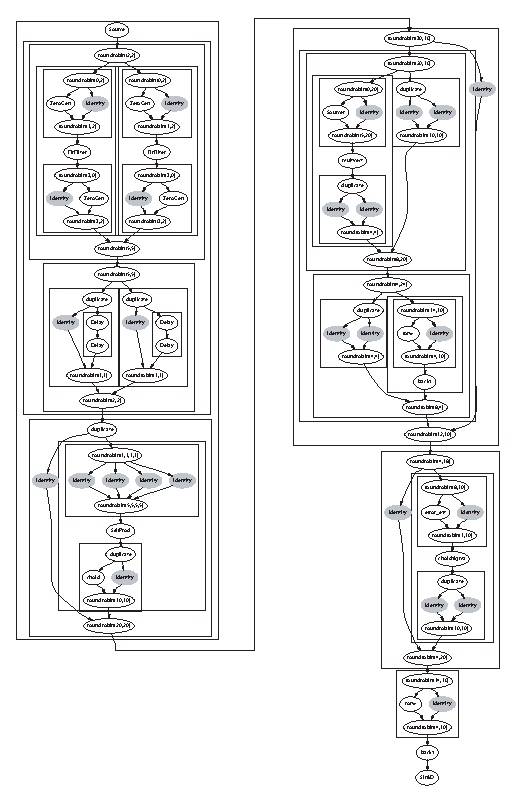
\psfig{file=3gpp.eps,height=\textheight}
%% \vspace{-0.9in} ~ \\
%% \mbox{~}\hspace{2.03in}\begin{minipage}{4in}
%% \caption[Use of Identity filters is illustrated by the 3GPP benchmark.]{Stream graph of a 3GPP Radio Access
%%   Protocol application.  Shaded filters indicate Identity nodes that
%%   are used to bypass data items around intermediate filters.  They are
%%   also used in splitjoins for data duplication and
%%   reordering.\protect\label{fig:3gpp}}
%% \end{minipage}
%% \end{figure*}

Needless to say, this pattern of multiplexing and demultiplexing adds
considerable complexity to the development process.  It requires the
programmer to maintain an unwritten contract regarding the logical
interleaving of data streams on each physical channel.  Moreover, the
addition of a new communication edge in the stream graph may require
modification to many intermediate stages.  We discuss possible
solutions and workarounds to this problem elsewhere~\cite{thies-thesis}.

%% While there is no perfect solution to this problem, we have
%% sometimes embraced two imperfect workarounds.  First, the data
%% items in the multiplexed streams can be changed from a primitive
%% type to a structure type, allowing each logical stream to carry its
%% own name.  This approach would benefit from a new kind of splitter
%% and joiner which automatically packages and un-packages structures
%% from adjoining data channels.  The second approach is to employ
%% teleport messaging, which allows point-to-point communication and
%% avoids interleaving stream data.  However, since it is designed for
%% irregular control messages, it does not expose information about
%% the steady-state dataflow to the compiler.

%% In practice, we have chosen to tolerate the occasional complexity
%% of stream multiplexing rather than to fall back on an unstructured
%% programming model.  However, it may be valuable to consider a
%% natural syntax for unstructured components of the stream graph --
%% the analog of break and continue statements (or even a rare GOTO
%% statement) in structured control flow. It is important to note,
%% however, that there is no overhead introduced by adding splitters
%% and joiners to the stream graph; the StreamIt compiler analyzes the
%% communication (via an analysis known as {\it synchronization
%% removal}) to recover the original unstructured communication.

Finally, there are rare cases in which the structured primitives in
StreamIt have been inadequate for representing a streaming
communication pattern.  Figure~\ref{fig:inadequate} illustrates an
example from video compression, where each parallel filter performs a
motion prediction for a fixed area of the screen.  Between successive
frames, each filters shares its prediction with its neighbors on
either side.  While this could be represented with a feedback loop
around the entire computation, there would be complicated interleaving
involved.
%This case reflects a broader shortcoming, discussed in
%Section~\ref{sec:lang-future-work}, that StreamIt is not designed for
%multidimensional data processing.

\begin{figure}[t]
\centering
\psfig{file=interleaving.eps,width=2.076in}

(a) Unstructured ~~~~~~ (b) Structured~~~~
\caption[Refactoring a stream graph to fit a structured programming
  model.]{Example of refactoring a stream graph to fit a structured
  programming model.  Both graphs achieve equivalent communication
  between filters.
\protect\label{fig:interleaving}}
\end{figure}

\begin{figure}[t]
\centering
\psfig{file=inadequate.eps,width=1.19in}

\caption[A communication pattern unsuitable for structured streams.]{A
  communication pattern unsuitable for structured streams.  This
  pattern can arise in video compression, where each block informs its
  neighbors of its motion prediction before the next processing
  step.\protect\label{fig:inadequate}}.
\end{figure}

% Programmers can accidentally introduce unnecessary mutable state in
% filters.
\myitem {\accidentalstate} Filters that have no mutable state are
attractive because they can be run in a data-parallel fashion.
Unfortunately, the performance cost of introducing state is not
exposed in the current StreamIt language.  Thus, we found that several
programmers, when faced with two alternative implementations of an
algorithm, would sometimes choose the one that includes mutable state.
Figure~\ref{fig:diff-stateful} gives a pedantic example of this
problem, while our accompanying report~\cite{thies-thesis} illustrates
a realistic case from MPD.  Prior to conducting our performance
evaluations, we examined all stateful filters in the benchmarks and
rewrote them as stateless filters when it was natural to do so.  In
future stream languages, it may be desirable to require an extra type
modifier on stateful filters, such as a {\it stateful} keyword in
their declaration, to force programmers to be cognizant of any added
state and to avoid it when possible.
\label{sec:accidentalstate}

%% \begin{figure*}[t]
%% \hspace{0.1\textwidth}
%% \begin{minipage}{0.35\textwidth}
%% \centering
%% \eightpoint
%% \begin{verbatim}
%% void->int filter SquareWave() {
%%   work push 2 {
%%     push(0);
%%     push(1);
%%   }
%% }
%% \end{verbatim}
%% \end{minipage}
%% \hspace{0.1\textwidth}
%% \begin{minipage}{0.35\textwidth}
%% \centering
%% \eightpoint
%% \begin{verbatim}
%% void->int filter SquareWave() {
%%   int x = 0;
 
%%   work push 1 {
%%     push(x);
%%     x = 1 - x;
%%   }
%% }
%% \end{verbatim}
%% \end{minipage}

%% \begin{minipage}{0.5\textwidth}
%% \centering
%% (a) Stateless
%% \end{minipage}
%% \begin{minipage}{0.5\textwidth}
%% \centering
%% (b) Stateful
%% \end{minipage}
%% \caption[Accidental introduction of filter state (pedantic example).]{Programmers 
%%   can accidentally introduce unnecessary filter state when writing
%%   programs.  In this example, the intended output is a square wave,
%%   emitting alternate values of 0 and 1.  Both implementations shown
%%   are functionally equivalent.  However, the stateless version (a)
%%   appears data-parallel to the compiler, while the stateful version
%%   (b) appears sequential.\protect\label{fig:state}}
%% \end{figure*}

%% \begin{figure*}[t]
%% \begin{minipage}{0.5\textwidth}
%% \centering
%% \eightpoint
%% \begin{verbatim}
%% float->float splitjoin 
%% CFARDelayToLMax_Stateless(int rows) {
%%     split roundrobin;
%%     add Delay(rows-1);
%%     add Delay(rows-1);
%%     add Identity<float>();
%%     add Delay(rows-1);
%%     add Delay(rows-1);
%%     join roundrobin;
%% }

%% float->float filter Delay(int N) {
%%     prework push N {
%%         for (int i=0; i<N; i++) {
%%             push(0.0);
%%         }
%%     }

%%     work push 1 pop 1 {
%%         push(pop());
%%     }
%% }
%% \end{verbatim}
%% \end{minipage}
%% \begin{minipage}{0.5\textwidth}
%% \centering
%% \eightpoint
%% \begin{verbatim}
%% float->float filter
%% CFARDelayToLMax_Stateful(int rows) {
%%     float[rows] guardNoise;
%%     float[rows] thresh;
%%     float[rows] sumDb;
%%     float[rows] guardDb;
%%     int popPos = 0;
%%     int pushPos = 1;

%%     work pop 5 push 5 {
%%         guardNoise[popPos] = pop();
%%         push(guardNoise[pushPos]);
%%         thresh[popPos] = pop();
%%         push(thresh[pushPos]);
%%         push(pop());
%%         sumDb[popPos] = pop();
%%         push(sumDb[pushPos]);
%%         guardDb[popPos] = pop();
%%         push(guardDb[pushPos]);

%%         popPos++;
%%         pushPos++;

%%         if(popPos >= rows) {
%%             popPos = 0;
%%         }
%%         if(pushPos >= rows) {
%%             pushPos = 0;
%%         }
%%     }
%% }
%% \end{verbatim}
%% \end{minipage}
%% ~ \\
%% \begin{minipage}{0.5\textwidth}
%% \centering
%% (a) Stateless
%% \end{minipage}
%% \begin{minipage}{0.5\textwidth}
%% \centering
%% (b) Stateful
%% \end{minipage}
%% \caption[Accidental introduction of filter state (real example).]{A 
%%   second example, drawn from MPD, in which a stateless computation was
%%   written in a stateful style in the original implementation.  The
%%   original version (b) performs a complex delay and reordering of
%%   interleaved vectors on the input stream, and appears stateful to the
%%   compiler.  It can be rewritten as a stateless construct (a), which
%%   separates the logical streams using a splitjoin and applies a
%%   stateless delay to each one.\protect\label{fig:state2}}
%% \end{figure*}

\myitem {\teleportmessaging} 
\label{sec:messaging}

As detailed in Table~\ref{tab:lang-messaging}, teleport messages are
utilized by four of the benchmarks (MPEG2 encoder, MPEG2 decoder,
Mosaic, and FHR).  There are a total of 8 logical messages, often
between multiple senders or multiple receivers.  Both upstream and
downstream messages are utilized; all messages are sent with a latency
of zero.  While relatively few of the benchmarks use teleport
messaging, the functionality provided is essential.  As described
elsewhere for the case of FHR~\cite{thies-ppopp05},
MPEG2~\cite{drake-thesis} and Mosaic~\cite{aziz-thesis}, messaging
simplifies and improves the expression of these algorithms in a
streaming context.
